\documentclass[a4paper,11pt]{article}
\usepackage{amsmath,amsthm,amsfonts,amssymb,amscd,amstext,vmargin,graphics,graphicx,tabularx,multicol} 
\usepackage[francais]{babel}
\usepackage[utf8]{inputenc}  
\usepackage[T1]{fontenc} 
\usepackage{pstricks-add,tikz,tkz-tab,variations}
\usepackage[autolanguage,np]{numprint} 

\setmarginsrb{1.5cm}{0.5cm}{1cm}{0.5cm}{0cm}{0cm}{0cm}{0cm} %Gauche, haut, droite, haut
\newcounter{numexo}
\newcommand{\exo}[1]{\stepcounter{numexo}\noindent{\bf Exercice~\thenumexo} : \marginpar{\hfill /#1}}
\reversemarginpar


\newcounter{enumtabi}
\newcounter{enumtaba}
\newcommand{\q}{\stepcounter{enumtabi} \theenumtabi.  }
\newcommand{\qa}{\stepcounter{enumtaba} (\alph{enumtaba}) }
\newcommand{\initq}{\setcounter{enumtabi}{0}}
\newcommand{\initqa}{\setcounter{enumtaba}{0}}

\newcommand{\be}{\begin{enumerate}}
\newcommand{\ee}{\end{enumerate}}
\newcommand{\bi}{\begin{itemize}}
\newcommand{\ei}{\end{itemize}}
\newcommand{\bp}{\begin{pspicture*}}
\newcommand{\ep}{\end{pspicture*}}
\newcommand{\bt}{\begin{tabular}}
\newcommand{\et}{\end{tabular}}
\renewcommand{\tabularxcolumn}[1]{>{\centering}m{#1}} %(colonne m{} centrée, au lieu de p par défault) 
\newcommand{\tnl}{\tabularnewline}

\newcommand{\bmul}[1]{\begin{multicols}{#1}}
\newcommand{\emul}{\end{multicols}}

\newcommand{\trait}{\noindent \rule{\linewidth}{0.2mm}}
\newcommand{\hs}[1]{\hspace{#1}}
\newcommand{\vs}[1]{\vspace{#1}}

\newcommand{\N}{\mathbb{N}}
\newcommand{\Z}{\mathbb{Z}}
\newcommand{\R}{\mathbb{R}}
\newcommand{\C}{\mathbb{C}}
\newcommand{\Dcal}{\mathcal{D}}
\newcommand{\Ccal}{\mathcal{C}}
\newcommand{\mc}{\mathcal}

\newcommand{\vect}[1]{\overrightarrow{#1}}
\newcommand{\ds}{\displaystyle}
\newcommand{\eq}{\quad \Leftrightarrow \quad}
\newcommand{\vecti}{\vec{\imath}}
\newcommand{\vectj}{\vec{\jmath}}
\newcommand{\Oij}{(O;\vec{\imath}, \vec{\jmath})}
\newcommand{\OIJ}{(O;I,J)}


\newcommand{\reponse}[1][1]{%
\multido{}{#1}{\makebox[\linewidth]{\rule[0pt]{0pt}{20pt}\dotfill}
}}

\newcommand{\titre}[5] 
% #1: titre #2: haut gauche #3: bas gauche #4: haut droite #5: bas droite
{
\noindent #2 \hfill #4 \\
#3 \hfill #5

\vspace{-1.6cm}

\begin{center}\rule{6cm}{0.5mm}\end{center}
\vspace{0.2cm}
\begin{center}{\large{\textbf{#1}}}\end{center}
\begin{center}\rule{6cm}{0.5mm}\end{center}
}



\begin{document}
\pagestyle{empty}
\titre{Interrogation sur les divisions euclidiennes }{Nom :}{Prénom :}{Classe}{Date}

\vspace*{0.5cm}

\begin{flushleft}
\begin{tabular}{|m{6cm}|m{2.5cm}|m{2.5cm}|m{2.5cm}|m{2.5cm}|}
\hline 
\textbf{Compétences} & \begin{center}
\textbf{Très bonne maîtrise}
\end{center} & \begin{center}
\textbf{Maîtrise satisfaisante}
\end{center}  & \begin{center}
\textbf{Maîtrise faible}
\end{center} & \begin{center}
\textbf{Maîtrise insuffisante}
\end{center} \\ 
\hline 
Je dois savoir calculer une division euclidienne &  &  & &\\
\hline
Je dois connaître et savoir utiliser le vocabulaire : dividende, diviseur, quotient et reste &  &  & & \\ 
\hline
Je dois connaître et savoir utiliser le vocabulaire : multiple, diviseur et divisible &  &  &  &\\ 
\hline 
Je dois connaître et savoir utiliser les critères de divisibilité par 2 ; 3 ; 4 ; 5 ; 9 ou 10  &  &  &  &\\ 
\hline 
Je dois savoir utiliser les mathématiques pour résoudre des problèmes issus de situations de la vie quotidienne  &  &  &  &\\ 
\hline   


\end{tabular} 
\end{flushleft}

\vspace*{0.75cm}

\exo{2,5}

\begin{center}
\includegraphics[scale=0.8]{divisioneuclidienne1.eps} 
\end{center}


\q Compléter les bulles avec le bon vocabulaire.\\

\q Effectuer cette division euclidienne\\

\vspace*{1cm}

\exo{2} Compléter les phrases avec le vocabulaire suivant : multiple,  diviseur ou divisible.      \\
 
 \bmul{2}
  35 est . . . . . . . . . . . . . . . de 7. \\
  
  4 et 9 sont  . . . . . . . . . . . . . . . . . 36.\\
  
  \columnbreak
  
  42 est . . . . . . . . . . . . . .  par le nombre 6. \\
  
  56 est . . . . . . . . . . . . . . . 8 et de 7 .\\
                                       
\emul

\newpage
   

\exo{2} Poser et effectuer les divisions euclidiennes. \\
Pour chaque division ci-dessous, \textbf{écrire l'égalité} vue dans le cours.\\


\hspace*{1.5cm} \qa 1716 $\div$ 3            \hspace*{6cm}                    \qa 7 869 $\div$ 75       \\

                        
\vspace*{5cm}

\exo{2}

Parmi les nombres suivants : 17 ; 233 ; 2115 ; 2523 ; 210 ; 468 ; 57\\

\bmul{2}

\initq \q	Quels sont ceux qui sont divisibles par 2 ?\\
\reponse[1]\\

\q	Quels sont ceux qui sont divisibles par 3 ?\\
\reponse[1]\\

\columnbreak

\q	Quels sont ceux qui sont divisibles par 4 ?\\
\reponse[1]\\

\q	Quels sont ceux qui sont divisibles par 9 ?\\
\reponse[1]\\

\emul

\exo{1,5} Pour le C.D.I. du collège, la documentaliste reçoit 370 livres qu'elle doit ranger sur des étagères. Elle ne peut transporter que 13 livres à la fois. \\

\initq \q Combien de voyages devra-t-elle faire au minimum ? \\
\reponse[4]\\

\q Combien de livres transportera-t-elle au dernier voyage ?\\
\reponse[2]\\



\exo{} Bonus : Labyrinthe\\

Trace le chemin pour aller de 1 à 180 sachant qu'on peut monter vers une brique qui contient un multiple ou descendre vers une brique qui
contient un diviseur, et qu'on ne peut pas se déplacer à l'horizontale.\\

\begin{center}
\includegraphics[scale=0.9]{labyrinthe.eps} 
\end{center}




\end{document}
